\subsection{Prior Predictive Distribution for $\tilde{\mu}^c$}
Here, we study the prior predictive distribution of $\tilde{\mu}^c$, the underlying 'true' value of the parameter $c$ for a patient with covariate vector $\tilde{x}$.  The goal of this section is to see how our prior belief on what $\tilde{\mu}^c$ varies depends on the hyperparameters.  We first describe the log-normal distribution, because it turns out this is the distribution that $\tilde{\mu}^c$ follows a log-normal distribution in the prior.

\subsubsection{Log-Normal Distribution}
A log-normal distribution is a continuous distribution defined on the open interval $(0, \infty)$.  A random variable $X$ follows a log-normal distribution if the transformed random variable $\log(X)$ follows a normal distribution.  An equivalent definition makes the parameterization of a log-normal distribution clear:

\begin{defn}
If $Y \sim \textrm{Normal}(\mu, \sigma^2)$, then the transformed random variable $X=\exp(Y)$ follows a $\textrm{Log-Normal}(\mu, \sigma^2)$ distribution.
\end{defn}

Thus, a Log-Normal distributed random variable $X$ is parameterized using the mean and standard deviation of the normal distribution that $\log(X)$ follows.

\subsubsection{Key Properties}

The density of a $\textrm{Log-Normal}(\mu, \sigma^2)$ distribution is:

\begin{eqnarray}
f_X(x;\mu, \sigma^2) = \frac{1}{x\sigma \sqrt{2\pi}} \exp{-\frac{(\log(x) - \mu)^2}{2 \sigma^2}};   x > 0
\end{eqnarray}

The log-normal distribution is unimodal regardless of the choice of parameters.  This is suitable for our poses.  There are analytical formulas for the mean and mode; the mean is $\exp(\mu + \frac{\sigma^2}{2)}$, and the mode is $\exp(\mu - \sigma^2)$.  Like in the case of the logit-normal distribution, neither the mean nor mode are constant as $\sigma^2$ increases, for fixed $\mu$.  Also, the mode and mean exhibit opposite trends.  Finally, as one would expect, the variance is increasing in $\sigma^2$.

\subsubsection{Log-Normality of $\tilde{\mu}^c$ in the Prior}

The only hyperparameter that $\tilde{\mu}^c$ depends on is $c^c$.  The argument for the log-normality of $\tilde{\mu}^c$ is exactly analogous to that for the logit-normality of $\tilde{\mu}^a$.  The prior predictive distribution of $\mu^c$, $\mu^c|c^c$, is distributed $g^c(\mu_{pop}^{c*} + B^c\tilde{x})$.  $B^c \sim N(0, c^cI)$, and so $B^c\tilde{x} \sim N(0, \tilde{\sigma}^c)$ where $\tilde{\sigma^c} := \tilde{x}'(c^cI)\tilde{x} = c^c\sum_{j=1}^k \tilde{x}_j^2$.  Thus $\mu_{pop}^{c*} + B^c\tilde{x} \sim N(\mu_{pop}^{c*}, \tilde{\sigma}^c)$ and thus $\tilde{\mu}^c \sim \textrm{log-normal}(\mu_{pop}^{c*}, \tilde{\sigma}^c)$.

\subsection{Choosing $c^c$ and $\lambda^c$}

As $P(\mu^c;c^c)$ is always unimodal, the only consideration we choosing $c^c$ is that if it is too large, the mean of $P(\mu^c;c^c)$ will shift too much as $\tilde{\sigma^c}$ changes.  We plotted the distribution of $P(\mu^c;c^c)$ for several values of $\mu_{pop}^c$ and $\tilde{\sigma}^c$.  From these plots, it seems that setting $c^c=1$ gives a distribution of $P(\mu^c;c^c)$ that does not shift too much with $\tilde{\sigma}^c$.

\begin{figure}
\begin{center}
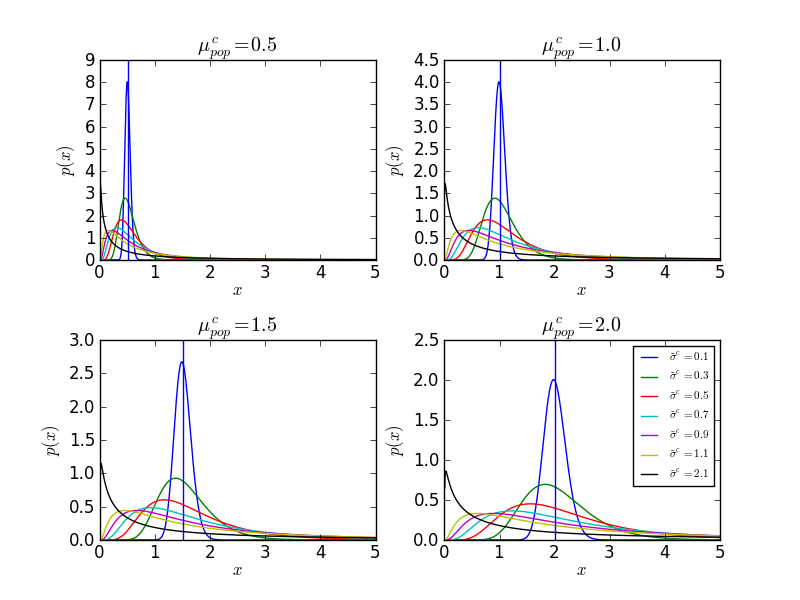
\includegraphics[width=3in, height=2in]{/Users/glareprotector/prostate_git/glare/tex_files/sections/gamma_prior/files/several_pdfs.png}
\caption{prior predictive distribution of $\tilde{\mu}^c$ for several values of $\mu_{pop}^c$ and $\tilde{\sigma}^c$}
\end{center}
\end{figure}

To choose $\lambda^c$, we once again need to encourage $\phi^c$ to be small.  We found that a value of $\lambda^c=1$, along with $c^c=1$, resulted in unimodal distributions for $P(\tilde{c}|c^c,\lambda^c)$.

\subsubsection{Choosing a prior for $\phi^{noise}$}
For the other parameters, we had to choose their corresponding hyperparmeters carefully because we desired that the prior of those parameters be unimodal.  However we don't run into such problems with choosing $\phi^{noise}$, as we know if the prior on $g(t;s,a,b,c)$ is unimodal, $g^*(g;s,a,b,c)$ will be unimodal regardless of the value of $\phi^{noise}$.  Then, we are free to estimate the hyperparameter for $\phi^{noise}$ from the data.  We can do so through maximum-likelihood estimation, jointly maximum all variables not conditioned on in the posterior, and seeing what the value of $\lambda^{noise}$ is.

\section{Plots of prior patient curve distributions}

Having established priors on all parameters by choosing values for the parameters, we have a prior predictive distribution $(P(a,b,c;\alpha,\tilde{X})$ where $\alpha$ denotes the hyperparameters.  Thus, we can plot the induced prior predictive distribution over 'true' curves, $P(g(t);s,a,b,c,\tilde{X})$, which we do so below, for several values of $\tilde{X}$.  Note that the curves are all centered approximately the same; the mode of the curve distribution is the same regardless of $\tilde{X}$.  However, their spread differs.  

\begin{figure}
\begin{center}
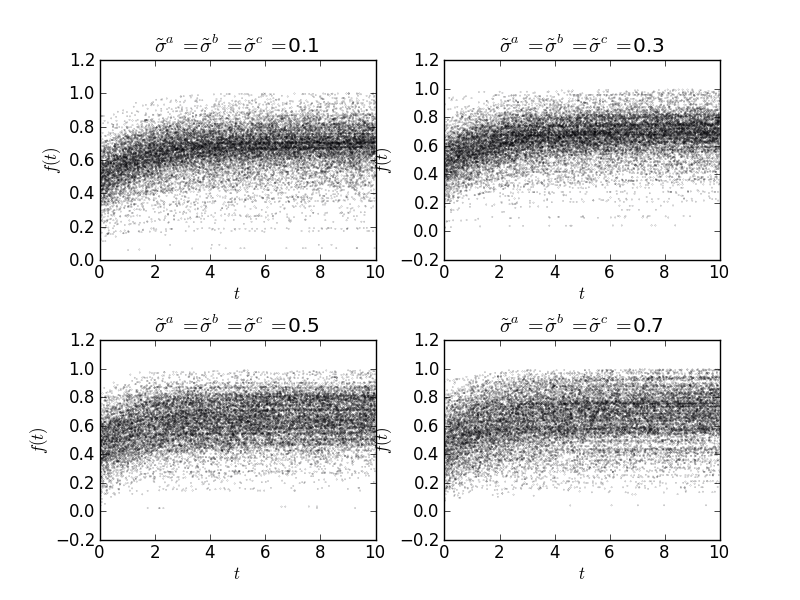
\includegraphics[width=3in, height=2in]{/Users/glareprotector/prostate_git/glare/tex_files/sections/curve_prior/files/curve_priors.png}
\caption{prior predictive distribution of over curves for several values of $\tilde{X}$}
\end{center}
\end{figure}